142. \begin{figure}[ht!]
\center{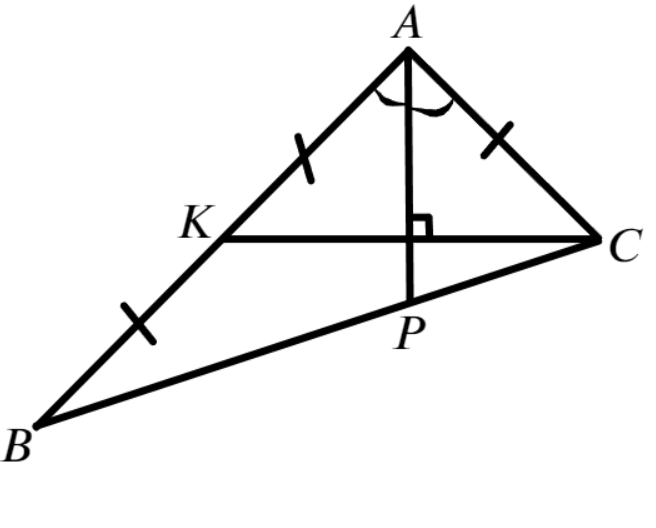
\includegraphics[scale=0.35]{g7-141.png}}
\end{figure}\\
Пусть биссектриса $AP$ перпендикулярна медиане $CK.$ Тогда в треугольнике $AKC$ биссектриса совпадает с высотой и он является равнобедренным, поэтому $AB=2AK=2AC.$ Обозначим стороны треугольника как $x,\ x+1$ и $x+2.$ Одна из его сторон оказалась в два раза больше другой. Если $x+1=2x,$ то $x=1, x+1=2,\ x+2=3,$ но для треугольника со сторонами 1, 2 и 3 не выполняется неравенство треугольника ($1+2=3$). Если $x+2=2x,$ то $x=2,\ x+1=3,\ x+2=4,$ для этого треугольника неравенство треугольника выполняется и его периметр равен $2+3+4=9.$ Если $x+2=2(x+1),$ то $x=0,$ что невозможно. Значит, периметр треугольника может быть равен только 9.\newpage\noindent
